\section{CAD modeling}
\label{sec:cad_modeling}

The first step in the analysis is to create the CAD of the model rocket.

Any CAD software can be used to create the model but for this project we used \texttt{CATIA V5}.

To simplify the analysis, some details of the rocket were omitted from the CAD model, such as the launch lug or the nozzle of the engine.
We believe that these simplifications do not affect the accuracy of the study, as the focus is on the nose cone, body, and fins of the rocket.

In Figure \ref{fig:CAD_model_drawing}, the technical drawing of the model is shown, along with the main dimensions.

\begin{figure}[H]
    \centering
    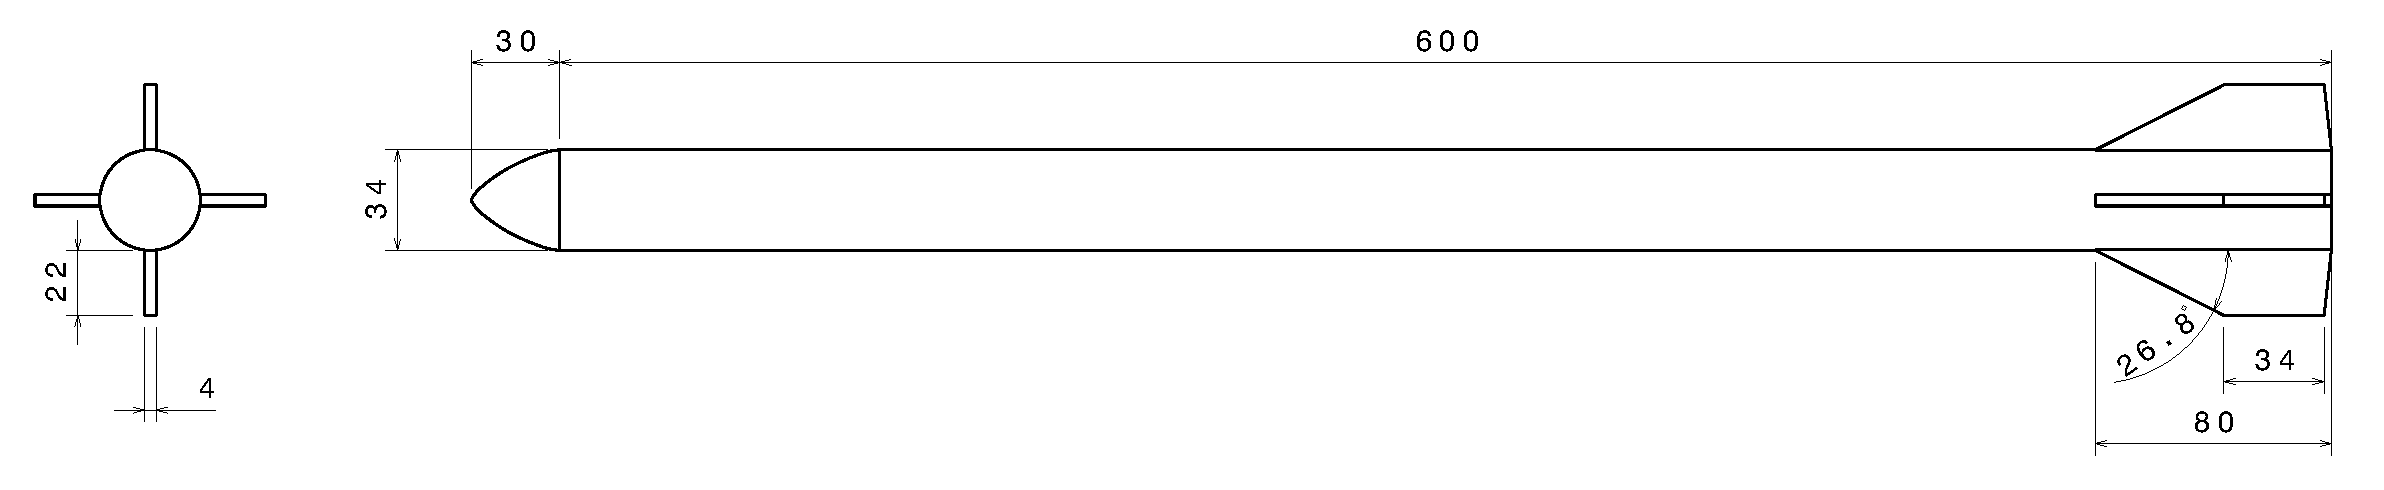
\includegraphics[width=\textwidth]{pdf/CAD_drawing.pdf}
    \caption{CAD model of the model rocket analyzed in this project. Measurements are in millimeters.}
    \label{fig:CAD_model_drawing}
\end{figure}

Probably the most important part of the CAD model is the choice of the nose cone shape.
For this project, we decided to adopt the \textbf{Haack series} nose cone, which is a common choice for model rockets.
In particular, instead of being geometrically defined, the Haack series nose cones are mathematically derived to minimize drag.
The shape is controlled by a parameter $C$, which can be set to different values to obtain different nose cone shapes.
The equations that defines the Haack series nose cone are:

\begin{align}
    \theta(x)    & = \arccos\left(1 - \frac{2x}{L}\right)                                            \\
    y(\theta, C) & = \frac{R}{\sqrt{\pi}} \sqrt{\theta - \frac{\sin{2\theta}}{2} + C \sin^3{\theta}} \\
\end{align}

Where $L$ is the length of the nose cone, $R$ is the radius of the base, and $C$ is the parameter that controls its shape.

In our case, we opted for a Haack series nose cone with $C = 0$, which is known to minimize the drag for a given length and diameter.
This choice is common in model rocketry, and can also be found under the name of \textbf{LD-Haack (Von Kármán)} nose cone.

\begin{figure}[H]
    \centering
    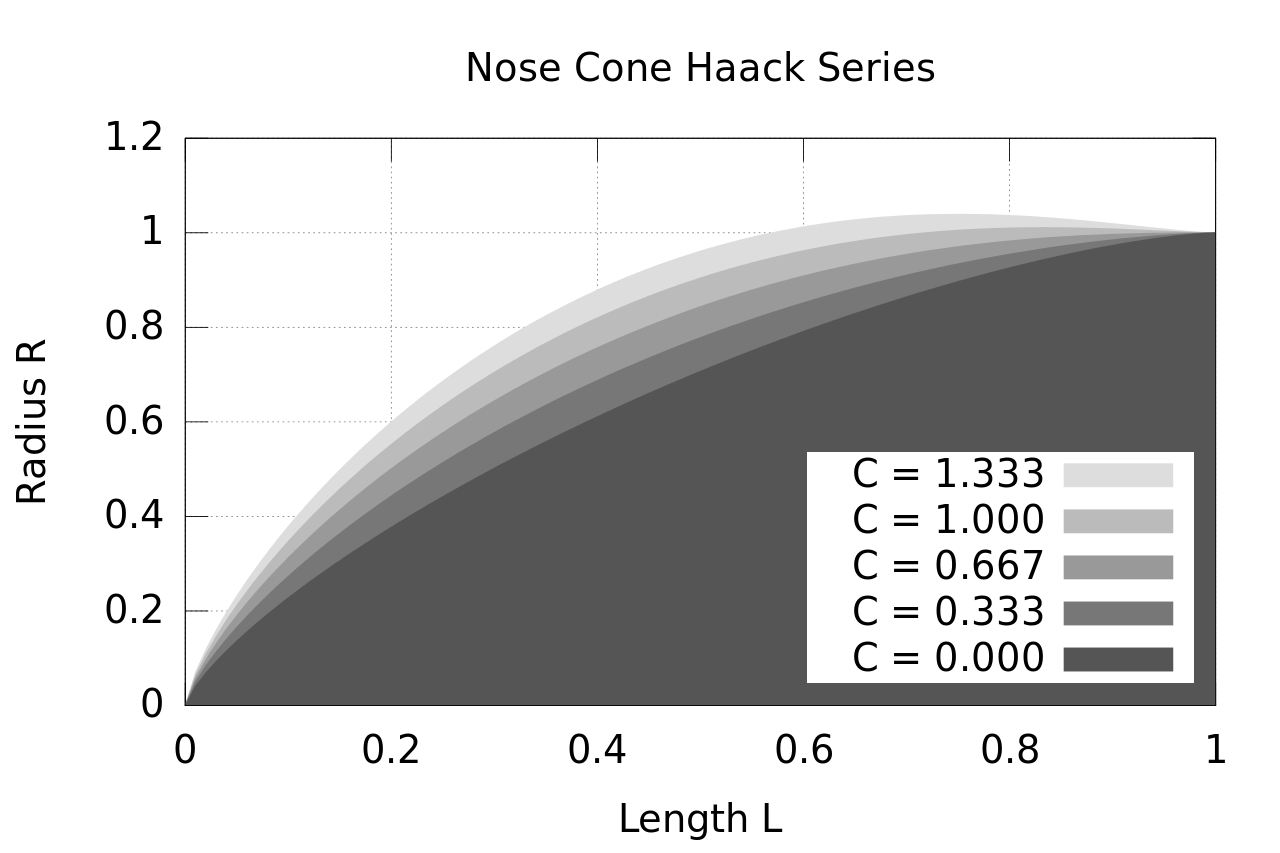
\includegraphics[width=.6\textwidth]{img/Nose_Cone_Haack_Series.png}
    \caption{Haack series nose cone with $L = 1$, $R = 1$, and different values of $C$.}
    \label{fig:LD_Haack_nose_cone}
\end{figure}